% Created 2016-05-15 Son 17:06
\documentclass[11pt, a4paper]{article}
\usepackage[utf8]{inputenc}
\usepackage[T1]{fontenc}
\usepackage{fixltx2e}
\usepackage{graphicx}
\usepackage{longtable}
\usepackage{float}
\usepackage{wrapfig}
\usepackage{soul}
\usepackage{textcomp}
\usepackage{marvosym}
\usepackage{wasysym}
\usepackage{latexsym}
\usepackage{amssymb}
\usepackage{hyperref}
\tolerance=1000
\usepackage{minted}
\usepackage[utf8]{inputenc}
\usepackage[english]{babel}
\usepackage{graphicx}
\usepackage[left=2.35cm, right=3.35cm, top=3.35cm, bottom=3.0cm]{geometry}
\usepackage{titling}
\providecommand{\alert}[1]{\textbf{#1}}

\title{Statistical methods for bioinformatics \linebreak GAM and Trees}
\author{Cedric Lood}
\date{\today}
\hypersetup{
  pdfkeywords={},
  pdfsubject={},
  pdfcreator={Emacs Org-mode version 7.9.3f}}

\begin{document}

\maketitle


\graphicspath{ {figures/} }
\setlength{\droptitle}{-5em} 
\setlength{\parindent}{0cm}

\section{Applied exercises}
\label{sec-1}
\subsection{Question 10}
\label{sec-1-1}

Libraries and definition of the training and test sets used for the
analysis:

\begin{minted}[]{R}
library(ISLR)
library(boot)
library(ggplot2)
library(leaps)
library(gam)

attach(College)
set.seed(1)
train <- sample(c(TRUE,FALSE), nrow(College), rep=TRUE)
test <- (!train)
\end{minted}
\subsubsection{Part a}
\label{sec-1-1-1}

The analysis reveals a forward selection with 6 variables retained in
the model:


\begin{minted}[]{R}
model.fwd <- regsubsets(Outstate~.,data=College[train,], nvmax=17,method="forward")
test.mat <- model.matrix(Outstate~., data=College[test,])

val.errors <- rep(NA, 17)
for(i in 1:17){
    coefi <- coef(model.fwd, id=i)
    pred <- test.mat[,names(coefi)] %*% coefi
    val.errors[i] <- mean((College$Outstate[test]-pred)^2)
}
val.errors
which.min(val.errors)
coef(model.fwd, 6)
\end{minted}


\begin{verbatim}
> val.errors
 [1] 10734659  7647452  6468424  5434378  4948421  4650921  4734848  4718857
 [9]  4690641  4735896  4694172  4877469  4754741  4690085  4711840  4700313
[17]  4700869
> which.min(val.errors)
[1] 6
> coef(model.fwd, 6)
  (Intercept)    PrivateYes    Room.Board      Terminal   perc.alumni 
-4227.6797221  2778.7052614     0.8106532    49.5653264    38.3960635 
       Expend     Grad.Rate 
    0.2616141    26.3975500
\end{verbatim}
\subsubsection{Part b}
\label{sec-1-1-2}

For this section, there are potentially many different GAM that could
be produced. For example, one could produce different functionals
consisting of smoothing splines for each of the predictors, with
different combinations of degrees of freedom. Here are a few, the
first one being akin to a multiple linear regression:


\begin{minted}[]{R}
model.gam <- gam(Outstate~Private+Room.Board+Terminal+perc.alumni+Expend+Grad.Rate,
                 data=College[train,])
pdf("gam_trees_s.pdf", width=16, height=12)
par(mfrow = c(3, 2))
plot.gam(model.gam,se=TRUE,col="green")
dev.off()

model.gam.s2 <- gam(Outstate~Private+s(Room.Board,df=2)+s(Terminal,df=2)+
                    s(perc.alumni,df=2)+s(Expend,df=2)+s(Grad.Rate,df=2),
                    data=College[train,])
pdf("gam_trees_s_2.pdf", width=16, height=12)
par(mfrow = c(3, 2))
plot.gam(model.gam.s,se=TRUE,col="green")
dev.off()

model.gam.s.3 <- gam(Outstate~Private+s(Room.Board,df=3)+s(Terminal,df=3)+
                     s(perc.alumni,df=3)+s(Expend,df=3)+s(Grad.Rate,df=3),
                     data=College[train,])
pdf("gam_trees_s_3.pdf", width=16, height=12)
par(mfrow = c(3, 2))
plot.gam(model.gam.s.3,se=TRUE,col="green")
dev.off()
\end{minted}

The graphics for the other 2 models can be found in the annex. Here
is the one for the smoothing splines with 2 degrees of freedom: 

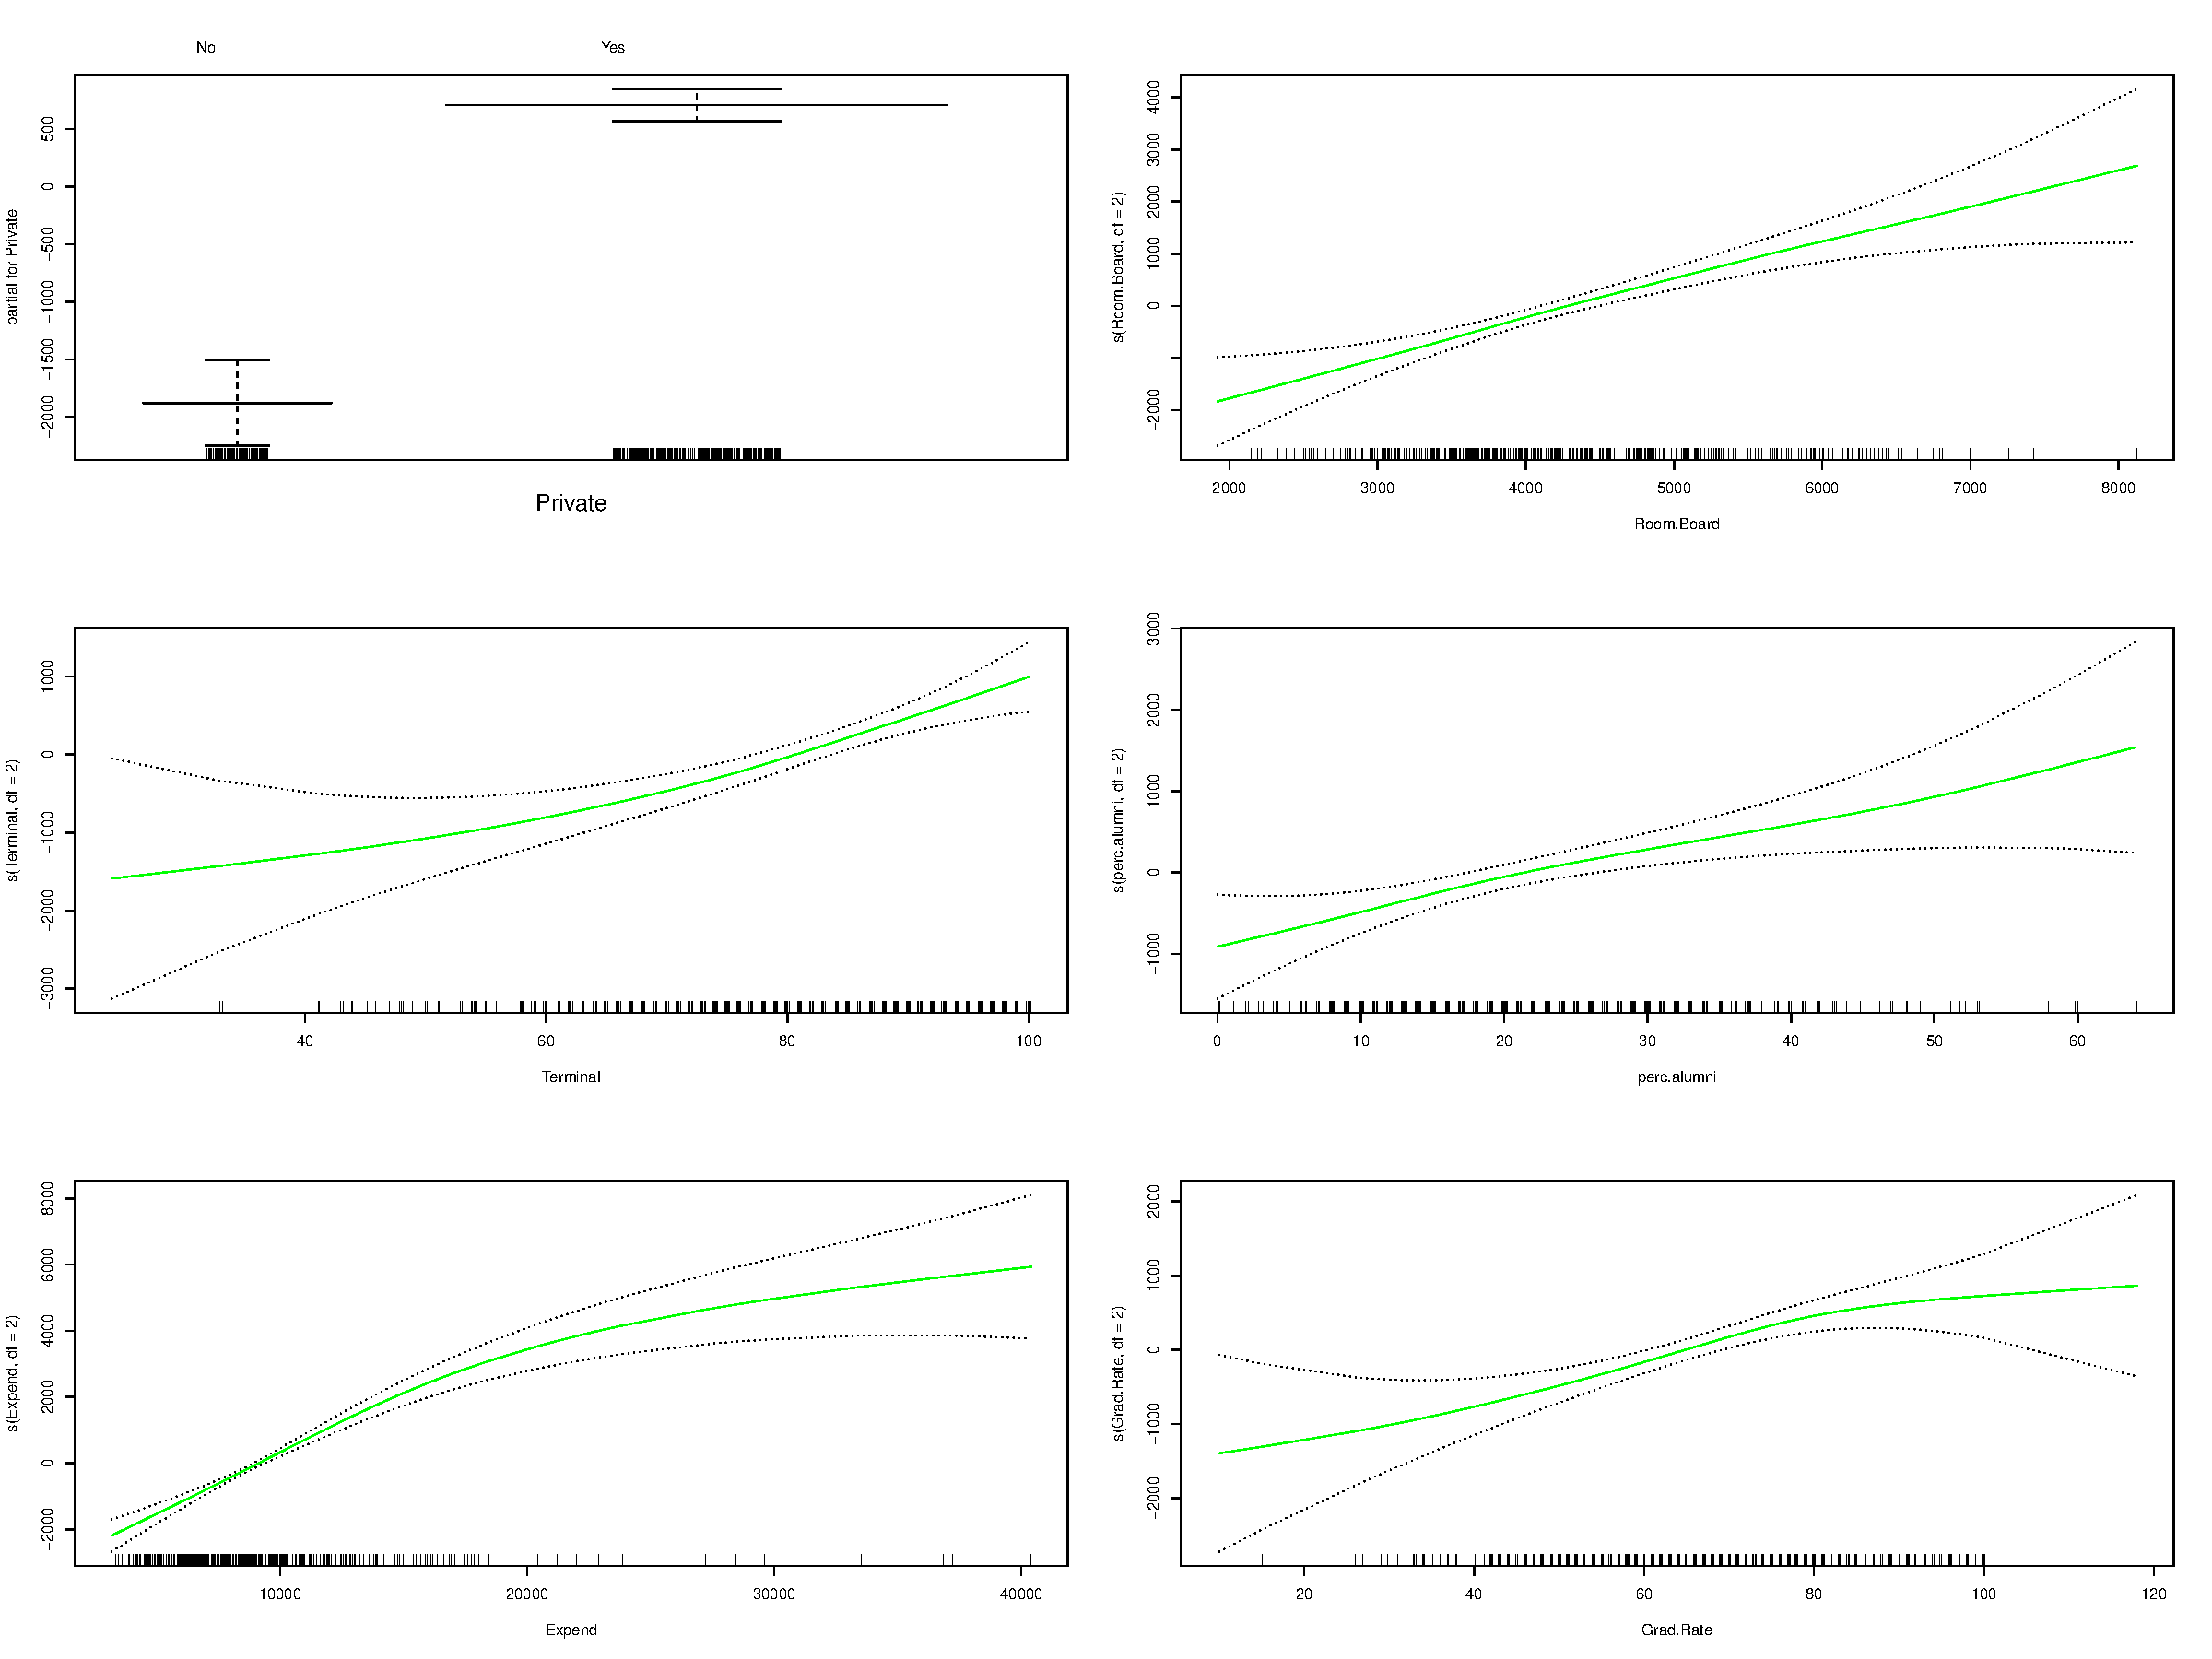
\includegraphics[scale=0.45]{gam_trees_s_2.pdf}
\subsubsection{Part c}
\label{sec-1-1-3}

This is the evaluation of the 3 different models for the test sets,
followed by the results. 


\begin{minted}[]{R}
gam.pred <- predict(model.gam,College[test,])
gam.err <- mean((College[test,]$Outstate - gam.pred)^2)

gam.pred.s2 <- predict(model.gam.s2,College[test,])
gam.err.s2 <- mean((College[test,]$Outstate - gam.pred.s2)^2)

gam.pred.s3 <- predict(model.gam.s.3,College[test,])
gam.err.s3 <- mean((College[test,]$Outstate - gam.pred.s3)^2)
\end{minted}


\begin{verbatim}
> gam.err
[1] 4650921
> gam.err.s2
[1] 3952853
> gam.err.s3
[1] 3784922
\end{verbatim}
\subsubsection{Part d}
\label{sec-1-1-4}

Evidence of non-linear relationship between variables can be
investigated using the summary function on the GAM. The function
provides the user with a non-parametric ANOVA table. Below is the
output of the command, which seem to indicate a non-linear
relationship between the predictor ``Expend'' and the dependent
value. 


\begin{verbatim}
> summary(model.gam.s2)

Call: gam(formula = Outstate ~ Private + s(Room.Board, df = 2) + s(Terminal, 
    df = 2) + s(perc.alumni, df = 2) + s(Expend, df = 2) + s(Grad.Rate, 
    df = 2), data = College[train, ])
Deviance Residuals:
    Min      1Q  Median      3Q     Max 
-7045.4 -1145.4    84.8  1184.1  5047.0 

(Dispersion Parameter for gaussian family taken to be 3452101)

    Null Deviance: 6006262152 on 405 degrees of freedom
Residual Deviance: 1360128366 on 394.0002 degrees of freedom
AIC: 7278.121 

Number of Local Scoring Iterations: 2 

Anova for Parametric Effects
                        Df     Sum Sq    Mean Sq F value    Pr(>F)    
Private                  1 1635387248 1635387248 473.737 < 2.2e-16 ***
s(Room.Board, df = 2)    1 1343549886 1343549886 389.198 < 2.2e-16 ***
s(Terminal, df = 2)      1  597441375  597441375 173.066 < 2.2e-16 ***
s(perc.alumni, df = 2)   1  240771844  240771844  69.746 1.161e-15 ***
s(Expend, df = 2)        1  424246993  424246993 122.895 < 2.2e-16 ***
s(Grad.Rate, df = 2)     1   63996091   63996091  18.538 2.104e-05 ***
Residuals              394 1360128366    3452101                      
---
Signif. codes:  0 ‘***’ 0.001 ‘**’ 0.01 ‘*’ 0.05 ‘.’ 0.1 ‘ ’ 1

Anova for Nonparametric Effects
                       Npar Df  Npar F     Pr(F)    
(Intercept)                                         
Private                                             
s(Room.Board, df = 2)        1  0.5670    0.4519    
s(Terminal, df = 2)          1  2.2148    0.1375    
s(perc.alumni, df = 2)       1  1.0512    0.3059    
s(Expend, df = 2)            1 26.1955 4.837e-07 ***
s(Grad.Rate, df = 2)         1  3.5803    0.0592 .  
---
Signif. codes:  0 ‘***’ 0.001 ‘**’ 0.01 ‘*’ 0.05 ‘.’ 0.1 ‘ ’ 1
\end{verbatim}
\subsection{Trees Vijver}
\label{sec-1-2}

Libraries and definition of the training dataset (126 cases out
of 188) used for the analysis.


\begin{minted}[]{R}
library(glmnet)
library(tree)
library(randomForest)
library(gbm)
library(ggplot2)

load("VIJVER.Rdata")
set.seed(1)
train <- sample(1:nrow(x), 126)
data.test <- data[-train,]
meta.test <- data$meta[-train]
\end{minted}
\subsubsection{Performance with Ridge and Lasso}
\label{sec-1-2-1}

For reminder, here are the performance obtained using regularization
techniques:


\begin{verbatim}
> perf.ridge
[1] 0.7580645
\end{verbatim}


\begin{verbatim}
> perf.lasso
[1] 0.6290323
\end{verbatim}
\subsubsection{Classification tree}
\label{sec-1-2-2}


\begin{minted}[]{R}
tree.data <- tree(meta~.,data=data,subset=train)
tree.pred <- predict(tree.data, data.test, type="class")
table(tree.pred, meta.test)
(15+25)/62 # perf=64.5%

pdf("tree_simple.pdf")
plot(tree.data)
text(tree.data, pretty=0)
dev.off()
\end{minted}


\begin{verbatim}
> table(tree.pred, meta.test)
         meta.test
tree.pred DM NODM
     DM   15    9
     NODM 13   25
> (15+25)/62
[1] 0.6451613
\end{verbatim}

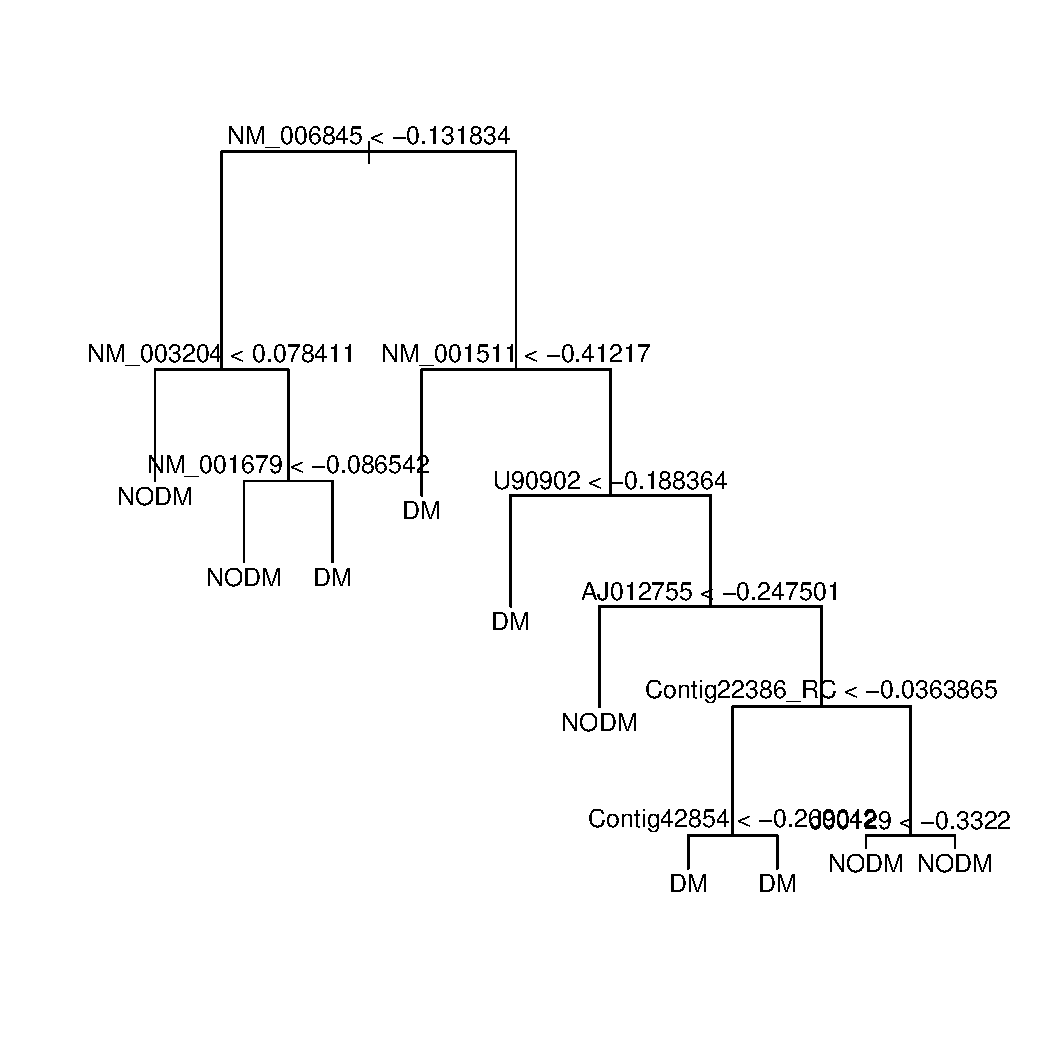
\includegraphics[scale=0.7]{tree_simple.pdf}
\subsubsection{Classification tree pruned}
\label{sec-1-2-3}

Prunning the tree results in a smaller tree at a very small penalty
in terms of predictive power (64\% -> 63\%)

\begin{minted}[]{R}
cv.data <- cv.tree(tree.data, FUN=prune.misclass)
cv.data # best depth=4
prune.data <- prune.misclass(tree.data, best=4)
tree.pred <- predict(prune.data, data.test, type="class")
table(tree.pred, meta.test)
(13+26)/62 # perf=63%

pdf("tree_pruned.pdf")
plot(prune.data)
text(prune.data, pretty=0)
dev.off()
\end{minted}


\begin{verbatim}
> 
         meta.test
tree.pred DM NODM
     DM   13    8
     NODM 15   26
> (13+26)/62 # perf=63%
[1] 0.6290323
\end{verbatim}

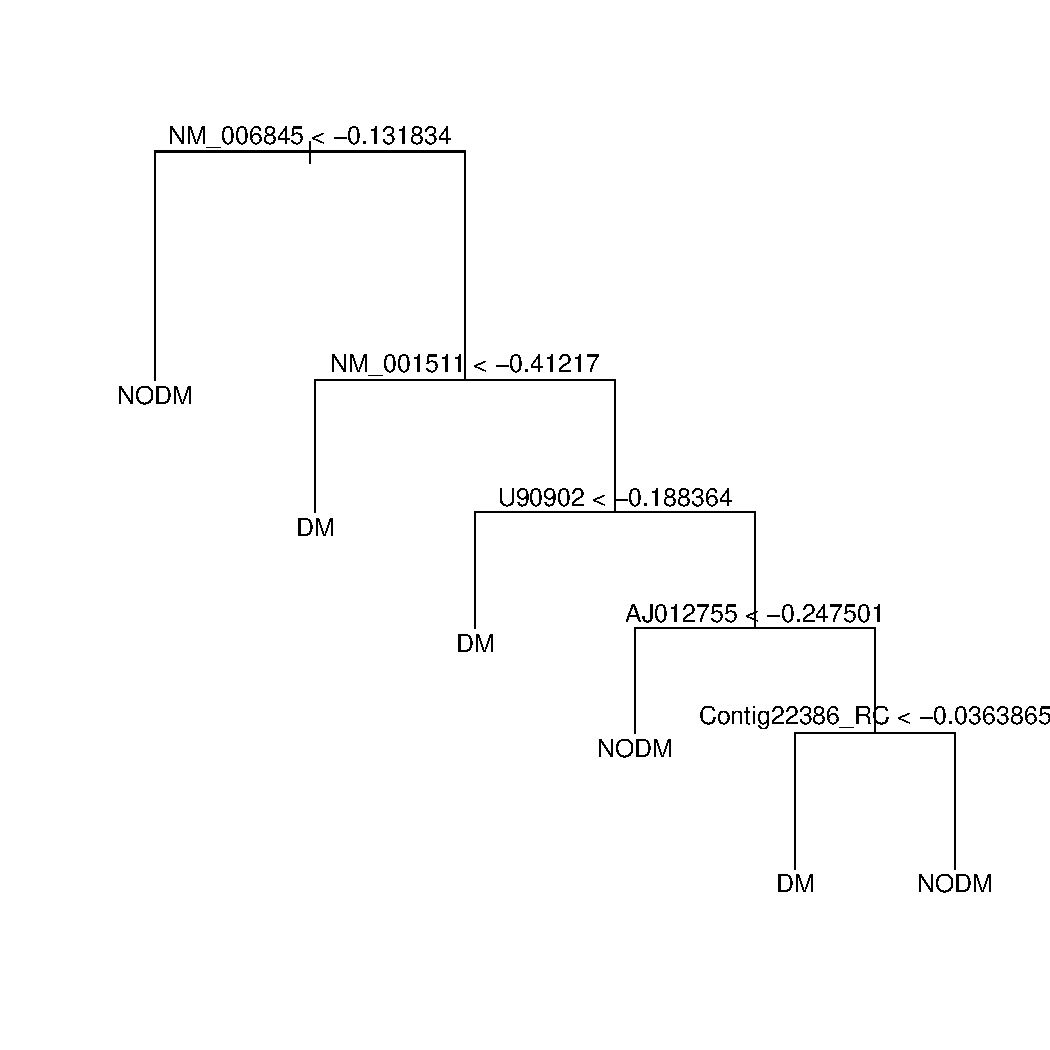
\includegraphics[scale=0.7]{tree_pruned.pdf}
\subsubsection{Intermezzo}
\label{sec-1-2-4}

For the techniques that follow, I used the variable selected by lasso
to proceed with the analysis. Trying to fit any of the ensemble
techniques, or boosting was not feasible on the full set of predictors
(about 5000) due to computational complexity. The variable selected
through lasso were:


\begin{verbatim}
> lasso.predictors
 [1] "NM_000918"      "NM_003258"      "NM_004119"      "AF279865"      
 [5] "NM_002811"      "Contig48919_RC" "NM_003714"      "NM_006054"     
 [9] "NM_007267"      "AF055033"       "Contig59134_RC" "NM_001007"
\end{verbatim}

And the definition of the datasets used for the next techniques:


\begin{minted}[]{R}
data.lasso <- data[c("meta", predictors.lasso)]
data.test <- data.lasso[-train,]
meta.test <- data.lasso$meta[-train]
\end{minted}

Of all these more advanced techniques, random forest obtained the
better score in terms of classification, with 68\% on the test
dataset. Followed by bagging (66\%) and boosting, which underperformed
the simpler tree established in the previous section.
\subsubsection{Bagging}
\label{sec-1-2-5}


\begin{minted}[]{R}
bag.data <- randomForest(meta~., data=data.lasso, subset=train, mtry=12, importance=TRUE)
yhat.bag <- predict(bag.data, newdata=data.test)
plot(yhat.bag, meta.test)
table(yhat.bag, meta.test)
(19+22)/62
importance(bag.data)
\end{minted}


\begin{verbatim}
> table(yhat.bag, meta.test)
        meta.test
yhat.bag DM NODM
    DM   18   11
    NODM 10   23
> (18+23)/62
[1] 0.6612903
\end{verbatim}

\includegraphics[scale=0.4]{}
\subsubsection{Random Forest}
\label{sec-1-2-6}


\begin{minted}[]{R}
rf.data <- randomForest(meta~., data=data.lasso, subset=train, importance=TRUE)
yhat.bag <- predict(rf.data, newdata=data.test)
plot(yhat.bag, meta.test)
table(yhat.bag, meta.test)
(19+24)/62
importance(rf.data)
\end{minted}


\begin{verbatim}
> table(yhat.bag, meta.test)
        meta.test
yhat.bag DM NODM
    DM   18   10
    NODM 10   24
> (18+24)/62
[1] 0.6774194
\end{verbatim}

\includegraphics[scale=0.4]{}
\subsubsection{Boosting}
\label{sec-1-2-7}


\begin{minted}[]{R}
## converting to binary (0,1) response
data.gbm <- data.lasso[,-1]
boolean <- ifelse(data.lasso$meta=="NODM", 1, 0)
data.gbm <- data.frame(boolean, data.gbm)
data.test <- data.gbm[-train,]

boost.data <- gbm(boolean~., data=data.gbm[train,], distribution="bernoulli",
                  n.trees=5000, interaction.depth=4)

yhat.boosting <- predict(boost.data, newdata=data.test, n.trees=100,distribution="bernoulli")
yhat.pred <- rep(0, 62)
yhat.pred[yhat.boosting>.5]=1
plot(yhat.boosting, data.test)
table(yhat.pred, boolean[-train])
(27+12)/62
\end{minted}


\begin{verbatim}
> table(yhat.pred, boolean[-train])
         
yhat.pred  0  1
        0 27 22
        1  1 12
> (27+12)/62
[1] 0.6290323
\end{verbatim}

\includegraphics[scale=0.4]{}
\subsubsection{Importance comparisons}
\label{sec-1-2-8}

As can be observed from the importance summary below, there isn't
much difference between random forest and bagging in terms of
importance of predictors. The order of the predictors in the case of
boosting was quite different.


\begin{minted}[]{R}
pdf("bag_data.pdf")
varImpPlot(bag.data)
dev.off()

pdf("rf_data.pdf")
varImpPlot(rf.data)
dev.off()

pdf("boost_data.pdf")
summary(boost.data)
dev.off()
\end{minted}


\begin{verbatim}
> importance(bag.data)
                       DM     NODM MeanDecreaseAccuracy MeanDecreaseGini
NM_000918       3.5037728 8.781774             9.182071         4.522524
NM_003258       7.1786980 6.169646             8.930712         6.413021
NM_004119       3.9275676 4.869651             6.053791         3.988813
AF279865       15.0288601 3.615650            13.997609         7.107205
NM_002811      12.8839394 5.005679            12.620362         6.377391
Contig48919_RC  7.8892269 8.526424            11.517478         6.630566
NM_003714       7.3136271 8.657350            10.483121         5.076347
NM_006054       3.3456481 5.128653             5.631485         3.451874
NM_007267       7.3468067 7.948700            10.334150         4.822468
AF055033        7.6168989 5.154784             8.312727         4.446796
Contig59134_RC -0.5793959 5.179788             3.915095         2.121363
NM_001007      10.9758645 4.700569            10.242585         4.866076

> importance(rf.data)
                      DM     NODM MeanDecreaseAccuracy MeanDecreaseGini
NM_000918       2.958896 8.473358             7.940691         4.716304
NM_003258       7.586545 7.203475            10.225379         6.139778
NM_004119       4.718333 4.904367             6.909594         4.366215
AF279865       12.520495 4.814431            11.358147         6.170585
NM_002811       8.764961 6.550887            10.304826         6.180394
Contig48919_RC  6.635444 7.277151             9.369255         5.369459
NM_003714       5.290677 5.371936             6.926086         4.734545
NM_006054       4.535794 3.973607             5.933265         3.849397
NM_007267       6.576916 7.798570             9.665736         5.724488
AF055033        8.064672 2.530757             6.983284         4.409412
Contig59134_RC  2.871751 4.405412             4.903617         3.420377
NM_001007       7.976717 6.581179             9.594289         4.901141

> summary(boost.data)
                          var   rel.inf
AF279865             AF279865 11.531043
NM_002811           NM_002811 10.949761
Contig48919_RC Contig48919_RC 10.296364
NM_007267           NM_007267  9.600293
NM_006054           NM_006054  8.549060
NM_001007           NM_001007  8.182846
NM_003258           NM_003258  8.075747
AF055033             AF055033  7.537565
NM_003714           NM_003714  7.276408
NM_000918           NM_000918  6.789771
NM_004119           NM_004119  6.271262
Contig59134_RC Contig59134_RC  4.939880
\end{verbatim}

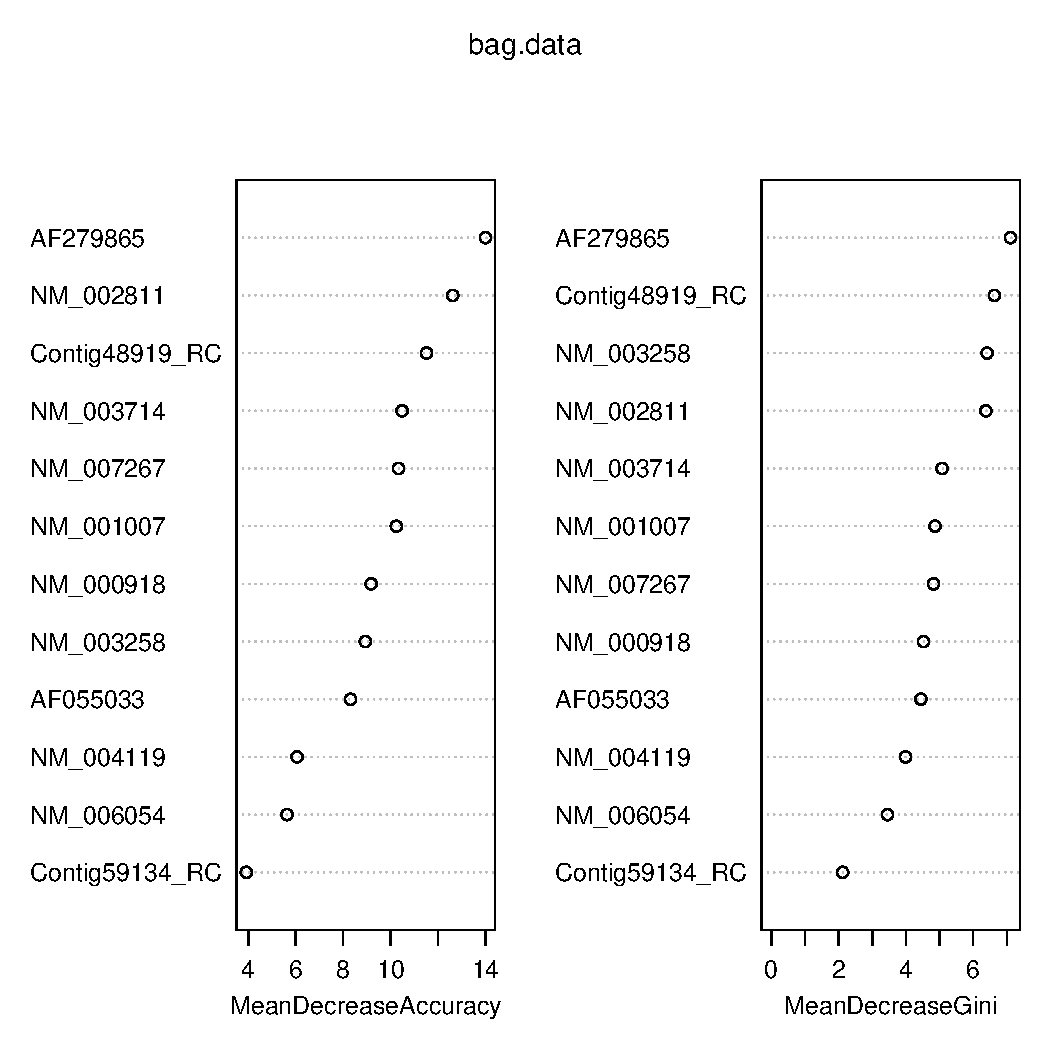
\includegraphics[scale=0.6]{bag_data.pdf}

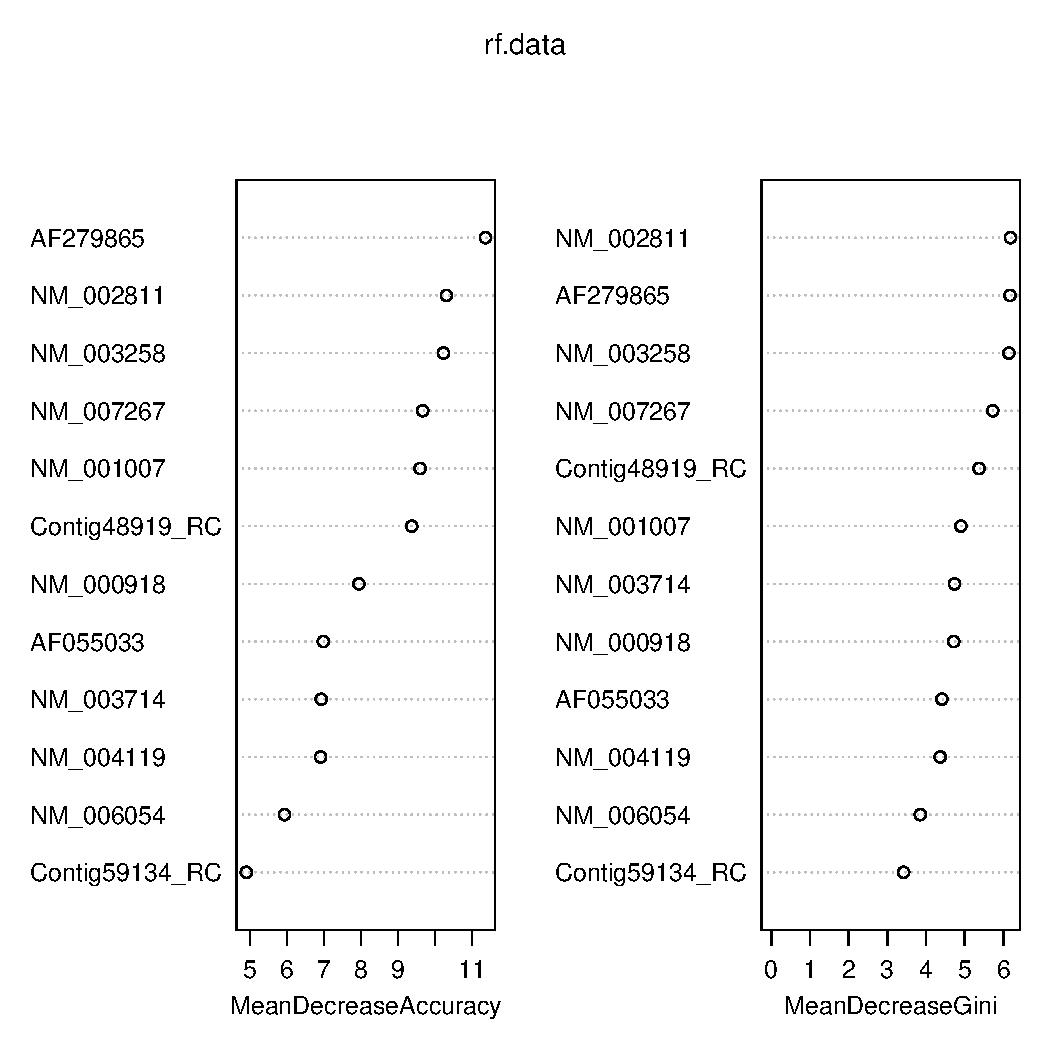
\includegraphics[scale=0.6]{rf_data.pdf}

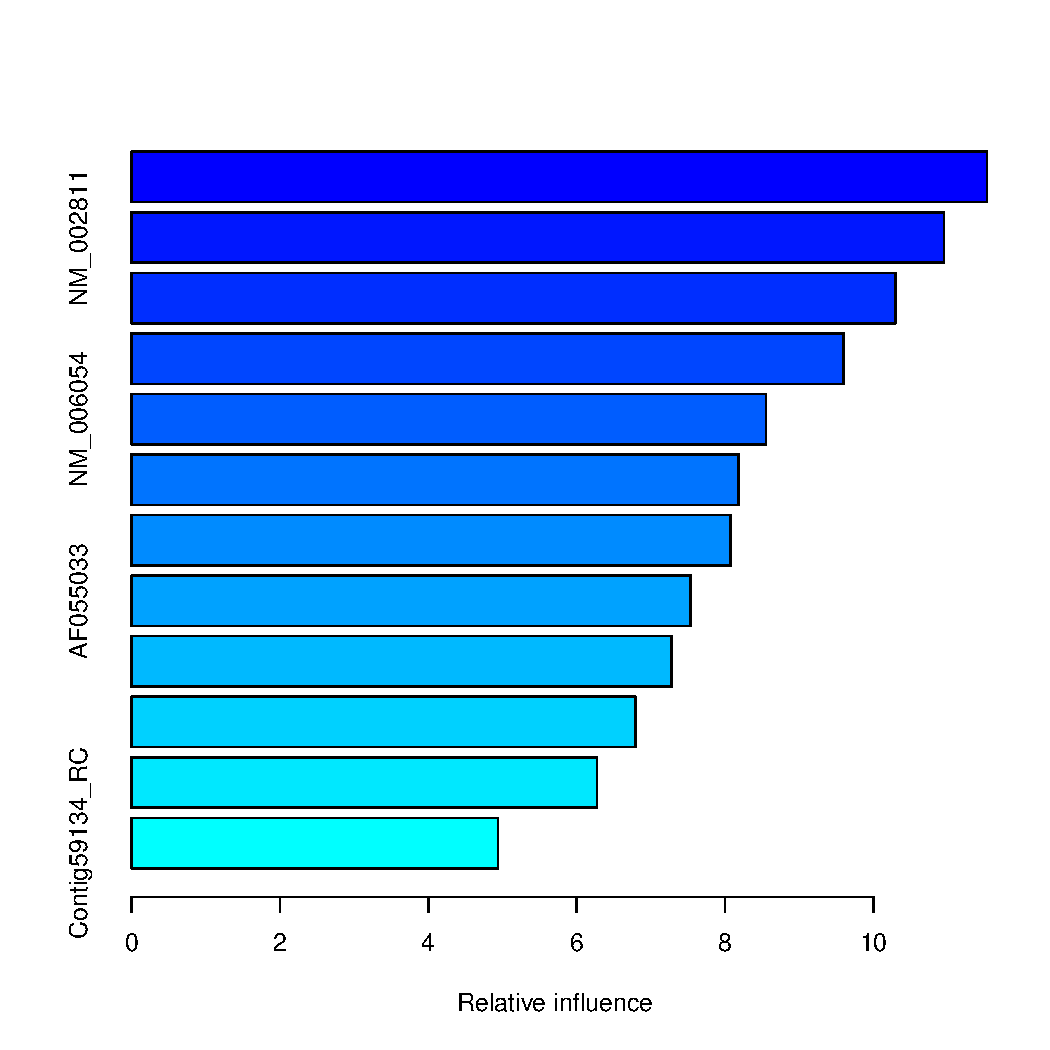
\includegraphics[scale=0.6]{boost_data.pdf}
\subsection{Annex}
\label{sec-1-3}

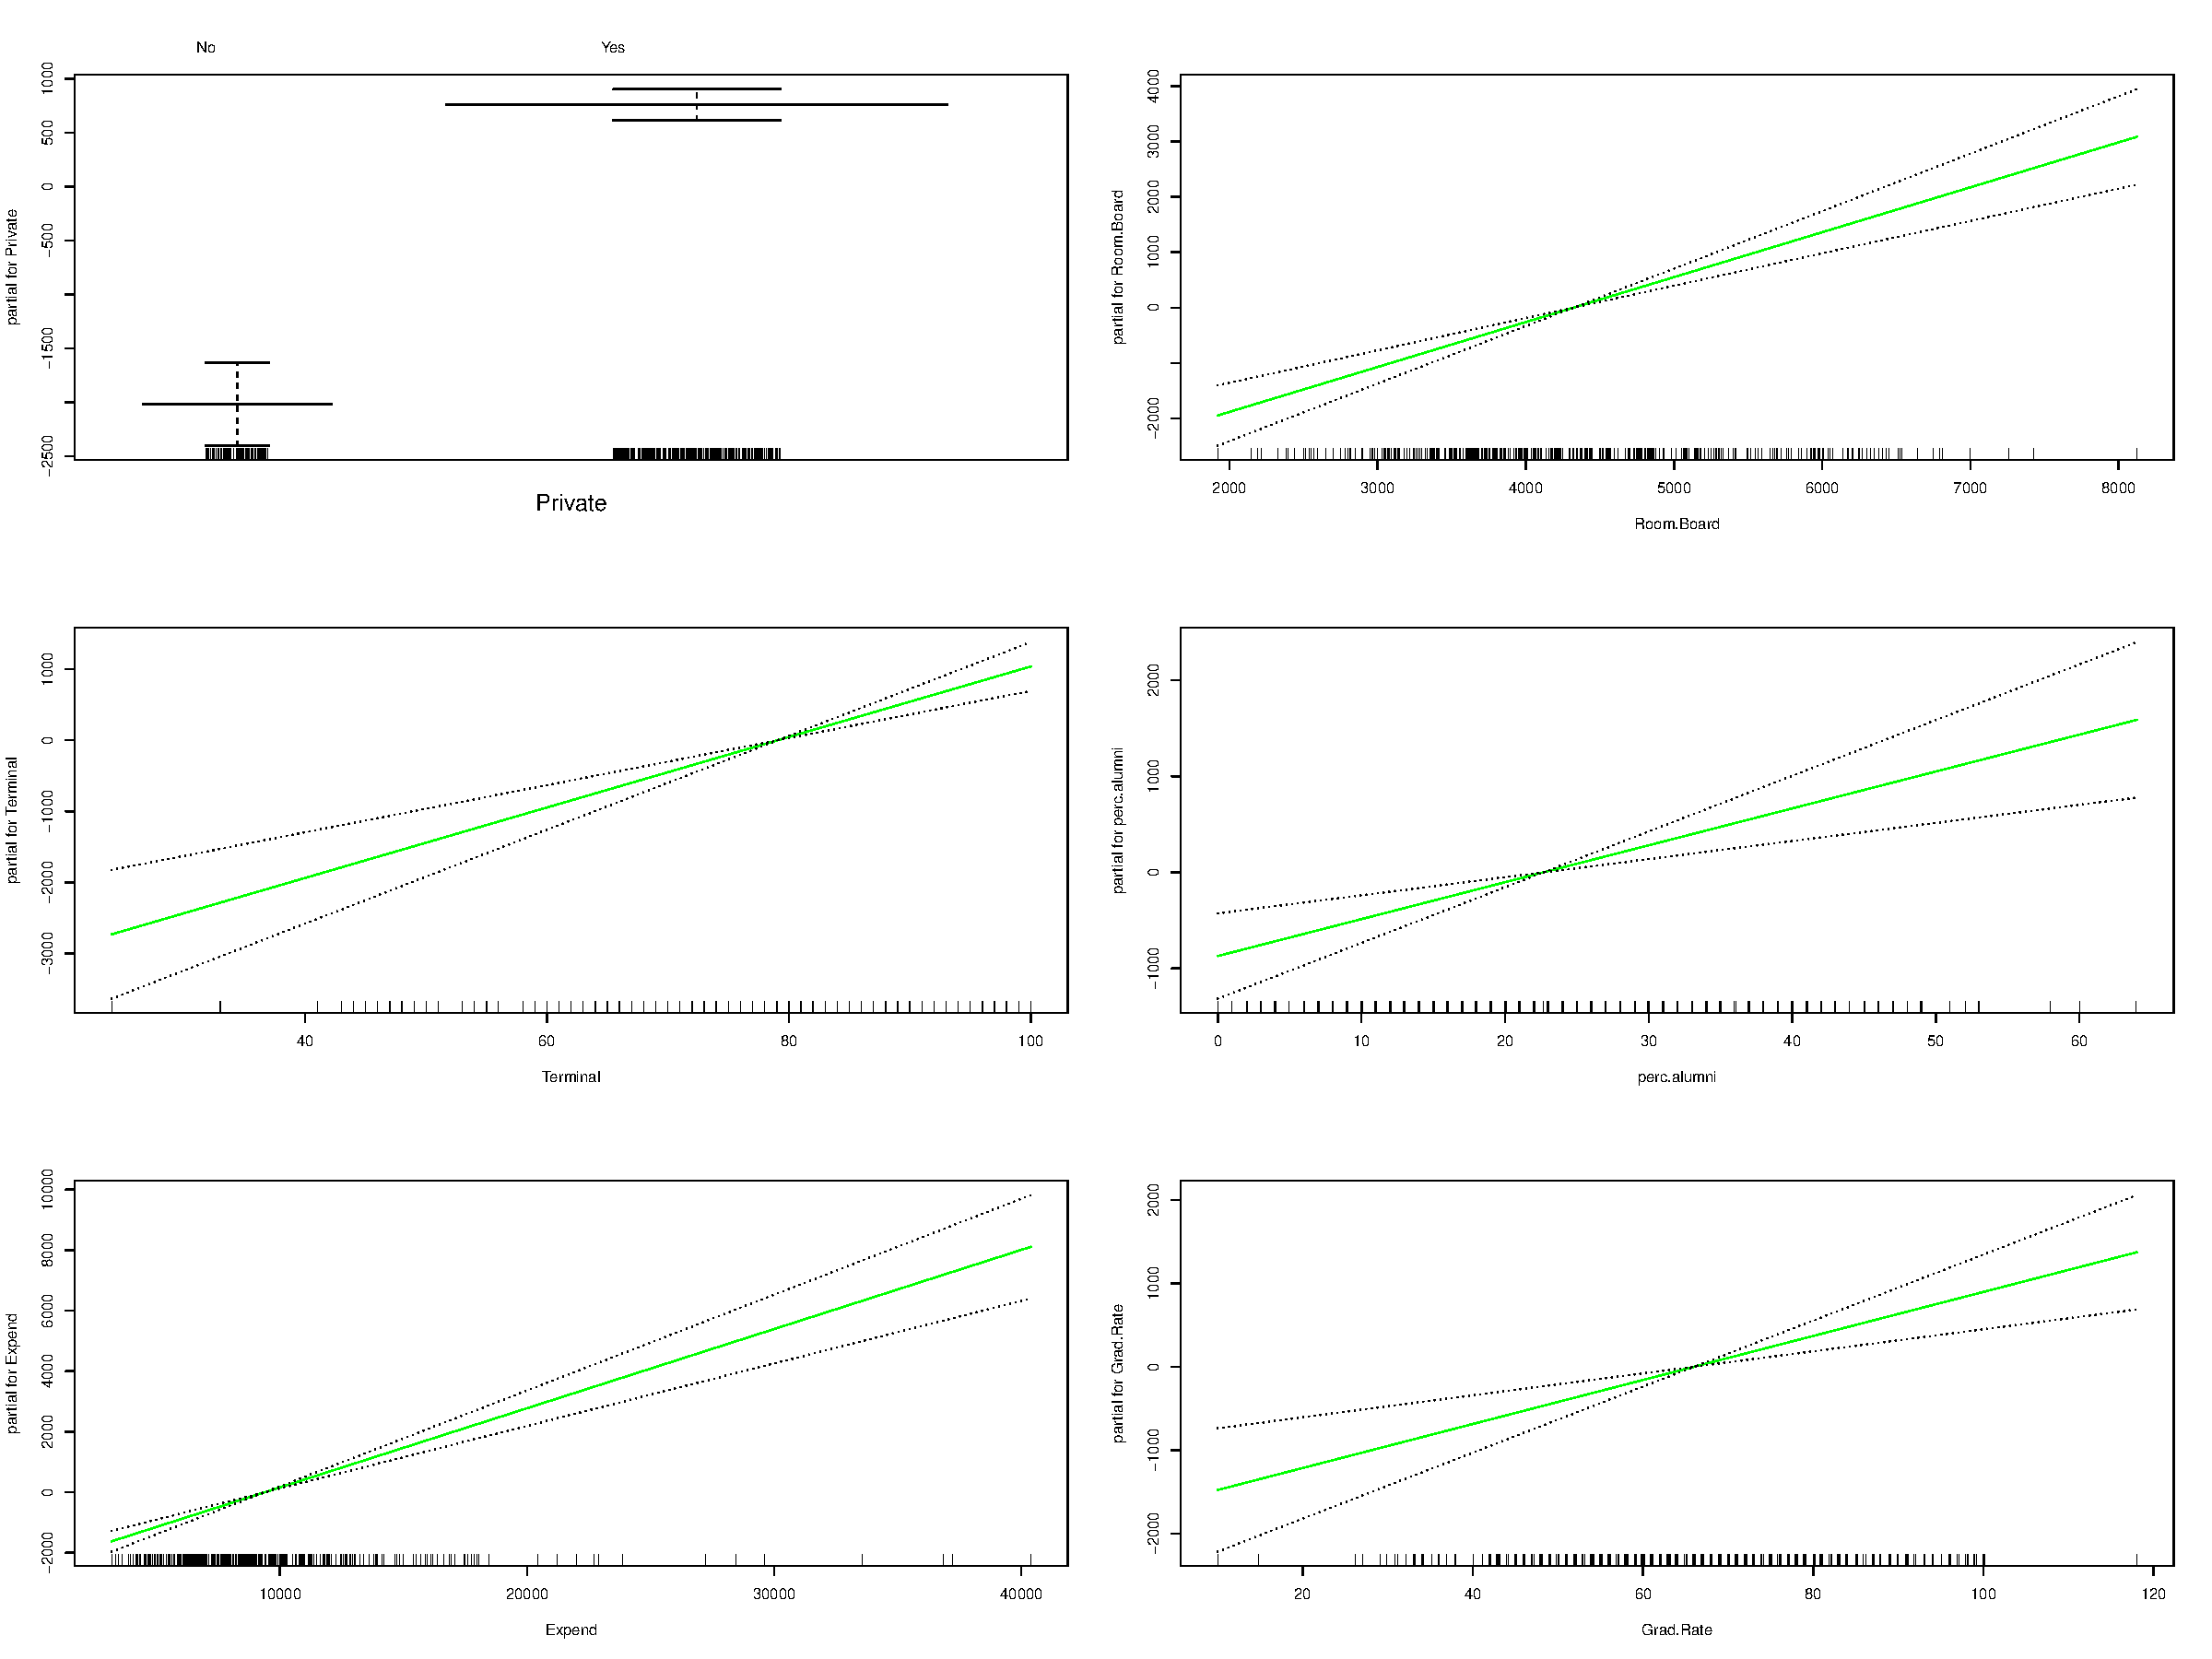
\includegraphics[scale=0.4]{gam_trees_s.pdf}

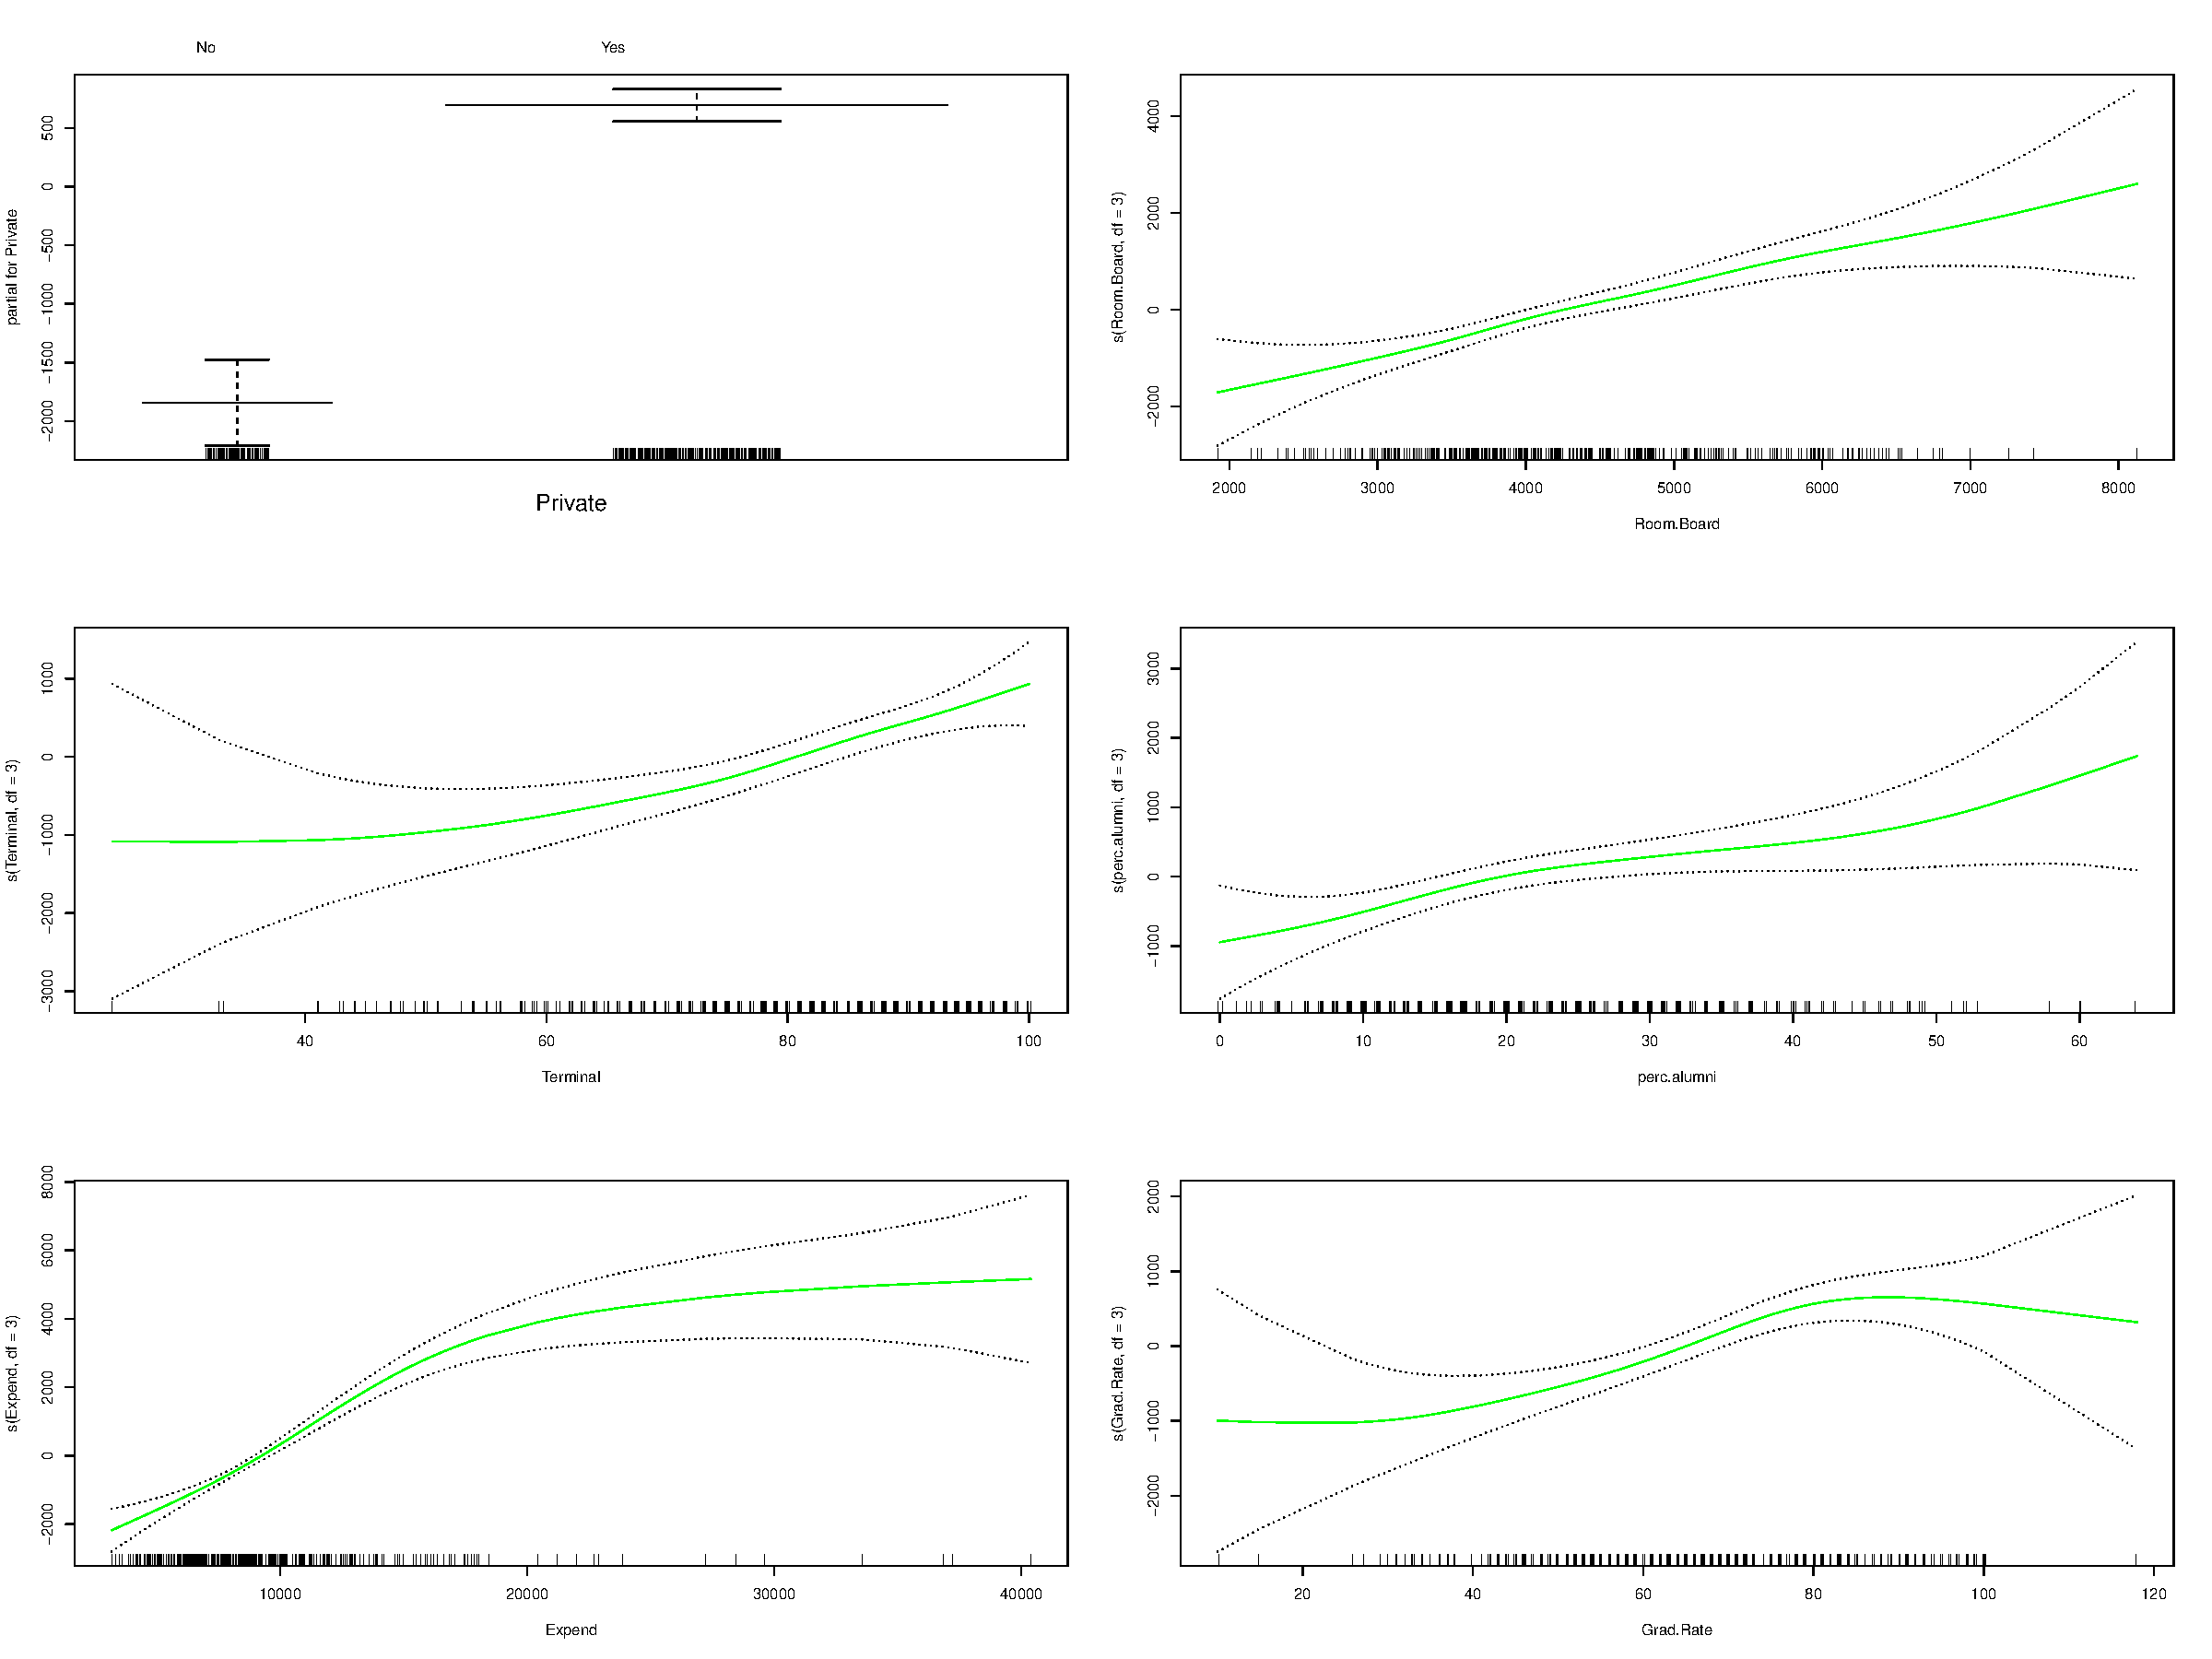
\includegraphics[scale=0.4]{gam_trees_s_3.pdf}

\end{document}
